\documentclass[usenames,dvipsnames,tikz]{standalone}
\usetikzlibrary{patterns}
%\usetikzlibrary{shapes.geometric}
%\usepackage{xcolor}
\colorlet{tBlue}{RoyalBlue!35!Cerulean}
\colorlet{tRed}{Red}
%\definecolor{tGreen}{HTML}{569909}
%\definecolor{tOrange}{HTML}{FA7602}
\usepackage{tikz}
\usepackage{standalone}
\begin{document}	
	
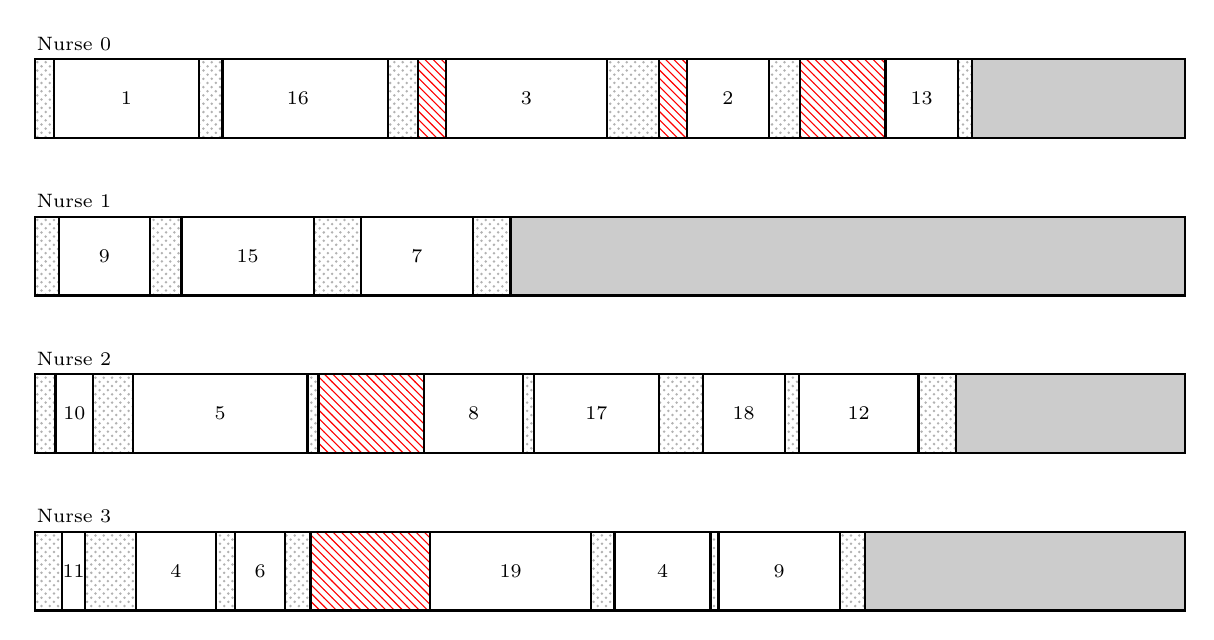
\begin{tikzpicture}
%\draw [help lines] (-1,-1) grid (15,8);

% Nurse 0
\draw [thick] (0,6) rectangle (14.6, 7);
\draw [thick, pattern = crosshatch dots, pattern color=black!30!white] (0,6) rectangle (0.24,7);
\draw [thick] (0.24,6) -- (0.24,7); % start of job 1
\draw [thick] (2.08,6) -- (2.08,7); % end of job 1
\draw [thick, pattern = crosshatch dots, pattern color=black!30!white] (2.08,6) rectangle (2.38,7);
\draw [thick] (2.38,6) -- (2.38,7); % start of job 16
\draw [thick] (4.48,6) -- (4.48,7); % end of job 16
\draw [thick, pattern = crosshatch dots, pattern color=black!30!white] (4.48,6) rectangle (4.86,7);
\draw [thick] (4.86,6) -- (4.86,7); % ARRIVE at job 3
\draw [thick, pattern = north west lines, pattern color=tRed] (4.86,6) rectangle (5.22,7);
\draw [thick] (5.22,6) -- (5.22,7); % start of job 3
\draw [thick] (7.26,6) -- (7.26,7); % end of job 3
\draw [thick, pattern = crosshatch dots, pattern color=black!30!white] (7.26,6) rectangle (7.92,7);
\draw [thick] (7.92,6) -- (7.92,7); % ARRIVE at job 2
\draw [thick, pattern = north west lines, pattern color=tRed] (7.92,6) rectangle (8.28,7);
\draw [thick] (8.28,6) -- (8.28,7); % start of job 2
\draw [thick] (9.32,6) -- (9.32,7); % end of job 2
\draw [thick, pattern = crosshatch dots, pattern color=black!30!white] (9.32,6) rectangle (9.72,7);
\draw [thick] (9.72,6) -- (9.72,7); % ARRIVE at job 13
\draw [thick, pattern = north west lines, pattern color=tRed] (9.72,6) rectangle (10.80,7);
\draw [thick] (10.80,6) -- (10.80,7); % start of job 13
\draw [thick] (11.72,6) -- (11.72,7); % end of shift
\draw [thick, pattern = crosshatch dots, pattern color=black!30!white] (11.72,6) rectangle (11.90,7);
\draw [thick] (11.90,6) -- (11.90,7); % end of shift
\draw [thick, fill=black!20!white] (11.90,6) rectangle (14.6,7);

\node [right] at (-0.1,7.2) {\scriptsize{Nurse 0}};
%\node at (1.16,6.6) {\scriptsize{job}}; 
%\node at (1.16,6.35) {\scriptsize{1}};
\node at (1.16,6.5) {\scriptsize{1}};
%\node at (3.34,6.6) {\scriptsize{job}};
%\node at (3.34,6.35) {\scriptsize{16}};
\node at (3.34,6.5) {\scriptsize{16}};
%\node at (6.24,6.6) {\scriptsize{job}};
%\node at (6.24,6.35) {\scriptsize{3}};
\node at (6.24,6.5) {\scriptsize{3}};
%\node at (8.80,6.6) {\scriptsize{job}};
%\node at (8.80,6.35) {\scriptsize{2}};
\node at (8.80,6.5) {\scriptsize{2}};
%\node at (11.26,6.6) {\scriptsize{job}};
%\node at (11.26,6.35) {\scriptsize{13}};
\node at (11.26,6.5) {\scriptsize{13}};


% Nurse 1
\draw [thick] (0,4) rectangle (14.6, 5);
\draw [thick, pattern = crosshatch dots, pattern color=black!30!white] (0,4) rectangle (0.30,5);
\draw [thick] (0.30,4) -- (0.30,5); % start of job 0
\draw [thick] (1.46,4) -- (1.46,5); % end of job 0
\draw [thick, pattern = crosshatch dots, pattern color=black!30!white] (1.86,4) rectangle (1.46,5);
\draw [thick] (1.86,4) -- (1.86,5); % start of job 15
\draw [thick] (3.54,4) -- (3.54,5); % end of job 15
\draw [thick, pattern = crosshatch dots, pattern color=black!30!white] (4.14,4) rectangle (3.54,5);
\draw [thick] (4.14,4) -- (4.14,5); % start of job 7
\draw [thick] (5.56,4) -- (5.56,5); % end of job 7
\draw [thick, pattern = crosshatch dots, pattern color=black!30!white] (6.04,4) rectangle (5.56,5);
\draw [thick] (6.04,4) -- (6.04,5); % end of shift
\draw [thick, fill=black!20!white] (6.04,4) rectangle (14.6,5);

\node [right] at (-0.1,5.2) {\scriptsize{Nurse 1}};
%\node at (0.88,4.6) {\scriptsize{job}}; 
%\node at (0.88,4.35) {\scriptsize{9}};
\node at (0.88,4.5) {\scriptsize{9}};
%\node at (2.70,4.6) {\scriptsize{job}}; 
%\node at (2.70,4.35) {\scriptsize{15}};
\node at (2.70,4.5) {\scriptsize{15}};
%\node at (4.85,4.6) {\scriptsize{job}}; 
%\node at (4.85,4.35) {\scriptsize{7}};
\node at (4.85,4.5) {\scriptsize{7}};



% Nurse 2
\draw [thick] (0,2) rectangle (14.6, 3);
\draw [thick, pattern = crosshatch dots, pattern color=black!30!white] (0,2) rectangle (0.26,3);
\draw [thick] (0.26,2) -- (0.26,3); % start of job 10
\draw [thick] (0.74,2) -- (0.74,3); % end of job 10
\draw [thick, pattern = crosshatch dots, pattern color=black!30!white] (0.74,2) rectangle (1.24,3);
\draw [thick] (1.24,2) -- (1.24,3); % start of job 5
\draw [thick] (3.46,2) -- (3.46,3); % end of job 5
\draw [thick, pattern = crosshatch dots, pattern color=black!30!white] (3.46,2) rectangle (3.60,3);
\draw [thick] (3.60,2) -- (3.60,3); % ARRIVE at job 8
\draw [thick, pattern = north west lines, pattern color=tRed] (3.60,2) rectangle (4.94,3);
\draw [thick] (4.94,2) -- (4.94,3); % start of job 8
\draw [thick] (6.20,2) -- (6.20,3); % end of job 8
\draw [thick, pattern = crosshatch dots, pattern color=black!30!white] (6.20,2) rectangle (6.34,3);
\draw [thick] (6.34,2) -- (6.34,3); % start of job 17
\draw [thick] (7.92,2) -- (7.92,3); % end of job 17
\draw [thick, pattern = crosshatch dots, pattern color=black!30!white] (7.92,2) rectangle (8.48,3);
\draw [thick] (8.48,2) -- (8.48,3); % start of job 18
\draw [thick] (9.52,2) -- (9.52,3); % end of job 18
\draw [thick, pattern = crosshatch dots, pattern color=black!30!white] (9.52,2) rectangle (9.70,3);
\draw [thick] (9.70,2) -- (9.70,3); % start of job 12
\draw [thick] (11.22,2) -- (11.22,3); % end of job 12
\draw [thick, pattern = crosshatch dots, pattern color=black!30!white] (11.22,2) rectangle (11.70,3);
\draw [thick] (11.70,2) -- (11.70,3); % end of shift
\draw [thick,fill=black!20!white] (11.70,2) rectangle (14.6,3);

\node [right] at (-0.1,3.2) {\scriptsize{Nurse 2}};
%\node at (0.50,2.6) {\scriptsize{job}}; 
%\node at (0.50,2.35) {\scriptsize{10}};
\node at (0.50,2.5) {\scriptsize{10}};
%\node at (2.35,2.6) {\scriptsize{job}}; 
%\node at (2.35,2.35) {\scriptsize{5}};
\node at (2.35,2.5) {\scriptsize{5}};
%\node at (5.57,2.6) {\scriptsize{job}}; 
%\node at (5.57,2.35) {\scriptsize{8}};
\node at (5.57,2.5) {\scriptsize{8}};
%\node at (7.13,2.6) {\scriptsize{job}}; 
%\node at (7.13,2.35) {\scriptsize{17}};
\node at (7.13,2.5) {\scriptsize{17}};
%\node at (9.00,2.6) {\scriptsize{job}}; 
%\node at (9.00,2.35) {\scriptsize{18}};
\node at (9.00,2.5) {\scriptsize{18}};
%\node at (10.46,2.6) {\scriptsize{job}}; 
%\node at (10.46,2.35) {\scriptsize{12}};
\node at (10.46,2.5) {\scriptsize{12}};


% Nurse 3
\draw [thick] (0,0) rectangle (14.6, 1);
\draw [thick, pattern = crosshatch dots, pattern color=black!30!white] (0,0) rectangle (0.34,1);
\draw [thick] (0.34,0) -- (0.34,1); % start of job 11
\draw [thick] (0.64,0) -- (0.64,1); % end of job 11
\draw [thick, pattern = crosshatch dots, pattern color=black!30!white] (0.64,0) rectangle (1.28,1);
\draw [thick] (1.28,0) -- (1.28,1); % start of job 4
\draw [thick] (2.30,0) -- (2.30,1); % end of job 4
\draw [thick, pattern = crosshatch dots, pattern color=black!30!white] (2.30,0) rectangle (2.54,1);
\draw [thick] (2.54,0) -- (2.54,1); % start of job 6
\draw [thick] (3.18,0) -- (3.18,1); % end of job 6
\draw [thick, pattern = crosshatch dots, pattern color=black!30!white] (3.18,0) rectangle (3.50,1);
\draw [thick] (3.50,0) -- (3.50,1); % ARRIVE at job 19
\draw [thick, pattern = north west lines, pattern color=tRed] (3.50,0) rectangle (5.02,1);
\draw [thick] (5.02,0) -- (5.02,1); % start of job 19
\draw [thick] (7.06,0) -- (7.06,1); % end of job 19
\draw [thick, pattern = crosshatch dots, pattern color=black!30!white] (7.06,0) rectangle (7.36,1);
\draw [thick] (7.36,0) -- (7.36,1); % start of job 4
\draw [thick] (8.58,0) -- (8.58,1); % end of job 4
\draw [thick, pattern = crosshatch dots, pattern color=black!30!white] (8.58,0) rectangle (8.68,1);
\draw [thick] (8.68,0) -- (8.68,1); % start of job 9
\draw [thick] (10.22,0) -- (10.22,1); % end of job 9
\draw [thick, pattern = crosshatch dots, pattern color=black!30!white] (10.22,0) rectangle (10.54,1);
\draw [thick] (10.54,0) -- (10.54,1); % end of shift
\draw [thick, fill=black!20!white] (10.54,0) rectangle (14.6,1);

\node [right] at (-0.1,1.2) {\scriptsize{Nurse 3}};
%\node at (0.49,0.6) {\scriptsize{job}}; 
%\node at (0.49,0.35) {\scriptsize{11}};
\node at (0.49,0.5) {\scriptsize{11}};
%\node at (1.79,0.6) {\scriptsize{job}}; 
%\node at (1.79,0.35) {\scriptsize{4}};
\node at (1.79,0.5) {\scriptsize{4}};
%\node at (2.86,0.6) {\scriptsize{job}}; 
%\node at (2.86,0.35) {\scriptsize{6}};
\node at (2.86,0.5) {\scriptsize{6}};
%\node at (6.04,0.6) {\scriptsize{job}}; 
%\node at (6.04,0.35) {\scriptsize{19}};
\node at (6.04,0.5) {\scriptsize{19}};
%\node at (7.97,0.6) {\scriptsize{job}}; 
%\node at (7.97,0.35) {\scriptsize{4}};
\node at (7.97,0.5) {\scriptsize{4}};
%\node at (9.45,0.6) {\scriptsize{job}}; 
%\node at (9.45,0.35) {\scriptsize{9}};
\node at (9.45,0.5) {\scriptsize{9}};






\end{tikzpicture}
	
\end{document}

%\draw [thick] (0,6) rectangle (6.95, 7);
%\draw [thick] (0.11,6) -- (0.11,7); % start of job 10
%\draw [thick] (0.99,6) -- (0.99,7); % end of job 10
%\draw [thick] (1.07,6) -- (1.07,7); % start of job 14
%\draw [thick] (1.7,6) -- (1.7,7); % end of job 14
%\draw [thick] (1.84,6) -- (1.84,7); % start of job 3
%\draw [thick] (2.86,6) -- (2.86,7); % end of job 3
%\draw [thick] (2.93,6) -- (2.93,7); % start of job 11
%\draw [thick] (3.4,6) -- (3.4,7); % end of job 11
%\draw [thick] (3.66,6) -- (3.66,7); % start of job 17
%\draw [thick] (4.64,6) -- (4.64,7); % end of job 17
%\draw [thick] (4.76,6) -- (4.76,7); % start of job 2
%\draw [thick] (5.08,6) -- (5.08,7); % end of job 2
%\draw [thick] (5.11,6) -- (5.11,7); % start of job 0 (DS)
%\draw [thick] (6.5,6) -- (6.5,7); % end of job 0 (DS)
%\draw [thick] (6.71,6) -- (6.71,7); % end of shift


